%-------------------------------------------------------------------------------------------------------
%-------------------------------------------------------------------------------------------------------
% Sec & Label

\section{Theoretical Analysis}
\label{sec:analysis}


%-------------------------------------------------------------------------------------------------------
%-------------------------------------------------------------------------------------------------------
% Intro

In this section, the circuit in Figure \ref{fig:Desenho_t2} is analysed theoretically.

Two methods were used and both will be explained and presented. In Subsection \ref{subsec:node_met}
the aplication of the mesh method and its results are shown. In Subsection \ref{subsec:node_met} the
same is done with the node method. \\

In both of these methods, three important equations were used: both Kirchhoff's laws (Kirchhof's
current law (KCL) - eq.(\ref{eq:kcl}) and Kirchhoff's voltage law (KVL) - eq.(\ref{eq:kvl}));
Ohm's law (eq.(\ref{eq:ohm})).

The algebraic sum of all the currents in any given node is zero:
\begin{equation}
	\sum I_i = 0
	\label{eq:kcl}
\end{equation}

The algebraic sum of all the voltages in any given closed-loop circuit (mesh) is zero:
\begin{equation}
	\sum V_i = 0
	\label{eq:kvl}
\end{equation}

The potential difference between the two nodes connected to a resistor is equal to the current that 
passes through the resistor multiplied by its resistance.
\begin{equation}
	V_i = R_iI_i
	\label{eq:ohm}
\end{equation}

\begin{figure}[ht]
	\centering
	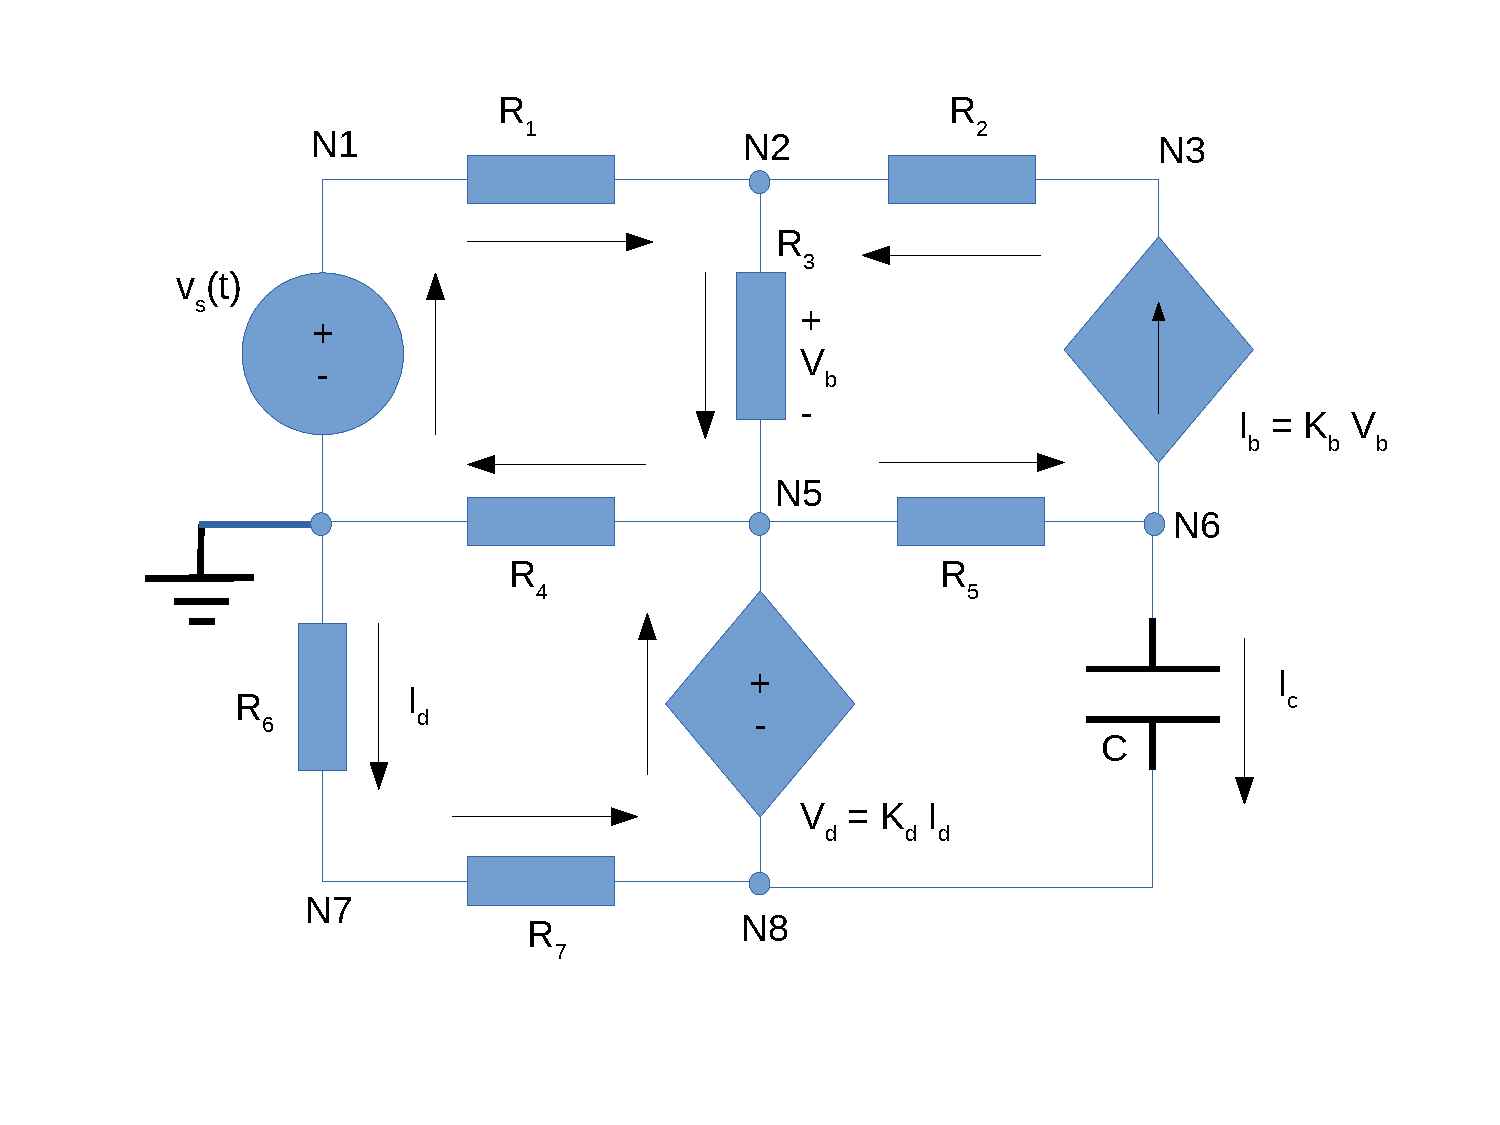
\includegraphics[width=0.85\linewidth]{dsnh_oct_t2.pdf}
	\caption{Circuit T2, node method}
\label{fig:Dsnh_oct_t2}
\end{figure}

%-----------------------------------------------------------------------
%-----------------------------------------------------------------------
% 			     Node - subsec
% ----------------------------------------------------------------------
% ----------------------------------------------------------------------

\subsection{Node method}
\label{subsec:node_met}


Similarly to the previous subsection, for the node method, ground was considered to be where it is identified in
Figure \ref{fig:Desenho_t2}. In adition, assume $V_{Ni}$ to be the voltage in node $Ni$ (every node position can
also be found in Figure \ref{fig:Desenho_t2}). \\

The node method uses KCL in conjunction with Ohm’s law to define equations that when solved give the voltage value 
of each nove in relation to ground (Node 0, $V_0 = 0$). In this circuit we defined six equations that equate the 
currents entering a particular node with the currents leaving said node. 

In order to have equations that solve for the node’s voltage, a relation between curent and voltage is made using 
Ohm’s law (given a resistance between two nodes, the current that passes the resistance can be written as 
$I=\frac{V_2-V_1}{R_1}$)

To simplify the equations it is useful to use the conductance $G_n$ which is the inverse of the resistance $R_n$ 
($G_n=\frac{1}{R_n}$)

\begin{equation}
	G_2(V_1-V_2)+G_1(V_3-V_2) - G3(V_2-V_4) = 0
	\label{}
\end{equation}

\begin{equation}
	G_2(V_1-V_2)+K_b(V_4-V_2) = 0
	\label{}
\end{equation}

\begin{equation}
	G3(V_2-V_4)+G_5(V_5-V_4)-G_4V_4)+I_c=0
	\label{}
\end{equation} 

\begin{equation}
	K_b(V_2-V_4)-G_5(V_5-V_4)=-I_d
	\label{}
\end{equation}

\begin{equation}
	G_7(V_6-V_7)-I_c=I_d
	\label{}
\end{equation}

\begin{equation}
	G_6(-V_6)-G_7(V_6-V_7)=0
	\label{}
\end{equation}

In order to solve the circuit two more equations are used to relate the voltage difference between the nodes that 
are conected to the voltage sources.

\begin{equation}
	V_3 = V_a
	\label{}
\end{equation}

\begin{equation}
	K_c\frac{(-V_6)}{G_6}-(V_4-V_7)=0
	\label{}
\end{equation}


With these 8 equations it is possible to solve the system using Octave.
The results were organized in Table \ref{tab:node}

\begin{table}[ht]
	\centering
	\begin{tabular}{|l|r|}
    		\hline    
    		{\bf Name} & {\bf Value [A or V]} \\ \hline
    		$V_{N1}$ & 5.114025e+00 \\ \hline 
$V_{N2}$ & 4.830792e+00 \\ \hline 
$V_{N3}$ & 4.226624e+00 \\ \hline 
$V_{N5}$ & 4.871651e+00 \\ \hline 
$V_{N6}$ & 5.781844e+00 \\ \hline 
$V_{N7}$ & -1.849204e+00 \\ \hline 
$V_{N8}$ & -2.786253e+00 \\ \hline 
$@I_{b}$ & -2.957272e-04 \\ \hline 
$@I_{c}$ & 0.000000e+00 \\ \hline 
$@I_{R1}$ & 2.822201e-04 \\ \hline 
$@I_{R2}$ & -2.957272e-04 \\ \hline 
$@I_{R3}$ & -1.350709e-05 \\ \hline 
$@I_{R4}$ & 1.200956e-03 \\ \hline 
$@I_{R5}$ & -2.957272e-04 \\ \hline 
$@I_{d}$ & -9.187358e-04 \\ \hline 
$@I_{R6}$ & 9.187358e-04 \\ \hline 

  	\end{tabular}
  	\caption{Values computed by Octave. Variables identified with a '$@$' have a
  	corresponding value in Ampere (A). The others are expressed in Volts (V).}
 
\label{tab:node}
\end{table}


